% ============================================================================
% NHQG solver: pedagogical review deck
%   Part A: the full numerical framework, as implemented (July 2026 state)
%   Part B: the aliased-vs-dealiased "blowup" of the stable runs, diagnosed:
%           the anti-Hermitian ky=0 ghost mode
% Build:  tectonic NHQG_framework_deck.tex
% ============================================================================
\documentclass[aspectratio=169,10pt]{beamer}
\usetheme{Boadilla}
\usecolortheme{default}
\setbeamertemplate{navigation symbols}{}
\setbeamertemplate{blocks}[rounded][shadow=false]
\usepackage{amsmath,amssymb}
\usepackage{booktabs}
\usepackage{tikz}
\usetikzlibrary{arrows.meta,positioning}

% ---- macros ---------------------------------------------------------------
\newcommand{\Rat}{\widetilde{Ra}}
\newcommand{\Ld}{L_d}
\newcommand{\Jac}[2]{J\!\left[#1,#2\right]}
\newcommand{\Tb}{\overline{\Theta}}
\newcommand{\avexy}[1]{\left\langle #1 \right\rangle_{xy}}
\newcommand{\dZ}{\partial_Z}
\newcommand{\lapp}{\nabla_{\!\perp}^{2}}
\newcommand{\file}[1]{\textcolor{blue!60!black}{\texttt{#1}}}
\newcommand{\Nud}{\mathrm{Nu}_{d}}
\newcommand{\Nuraw}{\mathrm{Nu}_{\mathrm{raw}}}

\title[NHQG framework \& the ghost-mode diagnosis]{The NHQG Solver, End to End}
\subtitle{Numerical framework $\;\bullet\;$ mean--fluctuation exchange $\;\bullet\;$
the aliased-vs-dealiased ``blowup'' diagnosed}
\author[NHQG review]{Pedagogical review deck \\ \small prepared with Claude Code}
\date{July 3, 2026}

\begin{document}

% ===========================================================================
\begin{frame}
  \titlepage
\end{frame}

\begin{frame}{Roadmap}
  \tableofcontents[hideallsubsections]
\end{frame}

% ===========================================================================
\section{Orientation: where the project stands}
% ===========================================================================

\begin{frame}{Timeline since you last looked (notes end mid-April)}
  \begin{itemize}
    \item \textbf{Apr 11--18} --- notes frozen: \file{blowup.md}, \file{adjoint\_mean\_exchange.md},
      \file{CLAUDE.md} status sections describe ``$t=80$ achieved at $64^2\times256$,
      coupling question open.''
    \item \textbf{Apr 19--20} --- scale-up campaign (post-dates all notes):
      \begin{itemize}
        \item $N_x{=}128,\ N_z{=}256$: clean to $\mathbf{t=120}$
          (\file{output\_combined\_Nx128\_Nz256\_...}), $\Nud\approx 19$--$22$.
        \item $N_x{=}256,\ N_z{=}256$: clean to $t=63$.
        \item Both: \texttt{balanced\_sbp2\_pc} + 4 corrector substeps + flux advection + 2/3-rule.
      \end{itemize}
    \item \textbf{May 19} --- run drivers updated (2/3-rule and \texttt{balanced\_sbp2\_pc} plumbing).
    \item \textbf{May 29} --- FD-vertical SBP42 campaign in \file{fd\_vertical\_benchmark/}
      (separate solver; targets the future mixed-BC goal). Last repo activity.
    \item \textbf{Jul 3 (this review)} --- 89/89 tests pass; the raw-diagnostics mystery
      of the stable runs is \emph{diagnosed} (Part B of this deck).
  \end{itemize}
  \begin{alertblock}{Operational summary}
    Late-time stability: \textbf{solved} (to $t=120$).\quad
    Raw-diagnostics ``blowup'': \textbf{explained} (ghost mode, Part B).\quad
    Physics validation: \textbf{open} ($\Nud\approx20$ vs.\ Miquel $43.4$ at $\Rat=100$).
  \end{alertblock}
\end{frame}

\begin{frame}{The physical problem}
  \begin{columns}[T]
    \column{0.58\textwidth}
    \textbf{Rapidly rotating Rayleigh--B\'enard convection} in the asymptotic
    limit $Ek\to 0$: the \emph{nonhydrostatic quasi-geostrophic equations}
    (NHQGE; Julien--Knobloch reduced dynamics).
    \begin{itemize}
      \item Ultimate target: \textbf{Jupiter's polar vortex crystals} (Juno) ---
        hence the $\beta$-effect and finite deformation radius $\Ld$ extensions,
        and later a polar-cap ``trap method'' (\file{NHGQ\_polar.tex}).
      \item Reference solution set: \textbf{Miquel et al.\ 2026}
        (tilted $f$-plane; $\vartheta_f=0^\circ$ reduces exactly to our system).
        Coral spectral code, IMEX RK443, Laplacian $\nu=1$ on all fields.
    \end{itemize}
    \column{0.40\textwidth}
    \begin{block}{Domain \& discretization at a glance}
      \begin{itemize}\itemsep2pt
        \item Horizontal: doubly periodic, $L\times L$ with $L=10\,L_c$,
          Fourier pseudospectral.
        \item Vertical: $Z\in[0,1]$, Chebyshev (CGL), Galerkin/tau.
        \item Time: ARS(2,2,2) IMEX--RK.
        \item JAX, GPU, float64.
      \end{itemize}
    \end{block}
  \end{columns}
\end{frame}

\begin{frame}{Governing equations (Miquel 3.1a--d, $\vartheta_f=0$, as implemented)}
  Four prognostic fields: $q'$ (PV perturbation), $w$, $\theta$, and the horizontal-mean
  temperature deviation $\Tb'(Z,t)$:
  \begin{align*}
    \partial_t q' + \Jac{\psi}{q'} + \beta\,\partial_x\psi
      &= \dZ w \;+\; \nu\lapp q' \\
    \partial_t w + \Jac{\psi}{w}
      &= -\dZ \psi \;+\; \tfrac{\Rat}{\sigma}\,\theta \;+\; \nu\lapp w \\
    \partial_t \theta + \Jac{\psi}{\theta}
      &= w\,\bigl(1 - \dZ\Tb'\bigr) \;+\; \tfrac{\nu}{\sigma}\lapp\theta \\
    \partial_t \Tb'
      &= \kappa_\theta\, \dZ^2 \Tb' \;-\; \mu\,\dZ\avexy{w\theta}
  \end{align*}
  \begin{itemize}
    \item Streamfunction by \emph{horizontal} inversion:
      $\hat\psi = -\hat q' / \bigl(|k|^2 + \Ld^{-2}\bigr)$, pointwise per Chebyshev coefficient.
    \item The $+w$ in the $\theta$ equation is conduction off the background $\Tb_{\rm tot}=1-Z$;
      the $-w\,\dZ\Tb'$ piece and the $-\mu\,\dZ\avexy{w\theta}$ piece are the
      \textbf{mean--fluctuation exchange pair} (Sec.~5) --- the crux of the last year.
    \item BCs: $w=\theta=0$ and $\Tb'=0$ at $Z=0,1$. \ $q'$ carries \textbf{no} BC
      (pure horizontal inversion of $\psi$; the March lesson).
    \item Coefficients $\mu,\kappa_\theta$: see \file{symbol\_map\_balanced\_sbp2\_pc.md}.
  \end{itemize}
\end{frame}

\begin{frame}{Parameters, onset, and validation targets}
  \begin{columns}[T]
    \column{0.5\textwidth}
    \begin{block}{Linear theory (stress-free)}
      \[
        s(k) = -\nu k^2 + \sqrt{\Rat - \pi^2/k^2}
      \]
      \begin{itemize}
        \item Onset: $\Rat_c \approx 8.6956$, $k_c \approx 1.3048$.
        \item At $\Rat=100$, $\nu=1$: max growth $\approx 8.6$ at $k\approx0.83$;
          unstable band $k \in (0.35,\, 3.16)$.
        \item \emph{Both numbers return in Part B --- remember them.}
      \end{itemize}
    \end{block}
    \column{0.48\textwidth}
    \begin{block}{Miquel Table 1 targets ($\vartheta_f=0$, $\sigma=1$)}
      \footnotesize
      \begin{tabular}{@{}rlrr@{}}
        \toprule
        $\Rat$ & grid & Nu & $Re_\ell$ \\
        \midrule
        40  & $128^2{\times}256$ & $12.28\pm0.60$ & $10.7$ \\
        80  & $128^2{\times}256$ & $30.96\pm1.81$ & $24.3$ \\
        100 & $256^2{\times}384$ & $\mathbf{43.37\pm2.54}$ & $32.1$ \\
        120 & $256^2{\times}384$ & $58.84\pm2.76$ & $41.2$ \\
        \bottomrule
      \end{tabular}
      \par\medskip
      \scriptsize Verified against the arXiv PDF. The copy in
      \file{experiments.md} is shifted by one row (row labels wrong); the
      \file{CLAUDE.md} copy is correct.
    \end{block}
  \end{columns}
  \medskip
  Production physics: $\Rat=100$, $\sigma=1$, $\beta=0$, $\Ld=\infty$,
  Laplacian $\nu=1$ on all fluctuation fields, no vertical diffusion on fluctuations.
\end{frame}

% ===========================================================================
\section{Spatial discretization}
% ===========================================================================

\begin{frame}{State representation: what is actually stored}
  \begin{center}
  \small
  \begin{tabular}{@{}llll@{}}
    \toprule
    field & basis & shape & BC handling \\
    \midrule
    $\hat q'$ & full Chebyshev coefficients & $(N_z{+}1,\,N_x,\,N_x/2{+}1)$ & none \\
    $\hat w$ & Dirichlet--Galerkin coefficients & $(N_z{-}1,\,N_x,\,N_x/2{+}1)$ & built into basis \\
    $\hat\theta$ & Dirichlet--Galerkin coefficients & $(N_z{-}1,\,N_x,\,N_x/2{+}1)$ & built into basis \\
    $\Tb'$ & Chebyshev coefficients (real) & $(N_z{+}1,)$ & tau rows \\
    \bottomrule
  \end{tabular}
  \end{center}
  \begin{itemize}
    \item Horizontal: \texttt{rfft2} layout --- real fields, half-plane storage
      $(N_x,\,N_k)$ with $N_k = N_x/2+1$. \emph{This layout carries implicit
      reality constraints; Part B is about what happens when they are violated.}
    \item Dirichlet--Galerkin basis (Coral's \texttt{bc\_type=20}):
      $\phi_n = -T_n + T_{n+2}$, which vanishes at $Z=0,1$ identically
      $\Rightarrow$ $w,\theta$ BCs are exact by construction, and the fields
      need only $N_z-1$ coefficients.
    \item \file{CLAUDE.md}'s top-level layout section still says $(N_z{+}1)$
      + tau rows for $w,\theta$ --- stale; the Coral-alignment restart note is the
      correct description.
  \end{itemize}
\end{frame}

\begin{frame}{Horizontal directions: Fourier pseudospectral}
  \begin{itemize}
    \item Doubly periodic box of side $L = 10 L_c \approx 48.15$;
      fundamental wavenumber $k_0 = 2\pi/L \approx 0.1305$.
    \item \texttt{rfft2}: a real $N_x\times N_x$ field $\mapsto$
      $(N_x,\ N_x/2{+}1)$ complex coefficients. Derivatives are diagonal:
      $\widehat{\partial_x f} = i k_x \hat f$.
    \item $\psi$ inversion is algebraic per mode:
      $\hat\psi = -\hat q'/(|k|^2 + \Ld^{-2})$ --- this is why $q'$ has no BC:
      the physical constraint $w=0$ at the walls acts on the $w$ equation
      (forcing $\dZ\psi=0$ there through the implicit coupling), not on $q'$.
    \item All nonlinear terms are quadratic (Jacobians / flux divergences),
      evaluated pseudospectrally $\Rightarrow$ \textbf{dealiasing} is required (Sec.~3).
  \end{itemize}
  \begin{block}{The one non-obvious fact about \texttt{rfft2} storage}
    The half-plane is not redundancy-free: the $k_y=0$ column (and the $k_y$-Nyquist
    column) must satisfy the self-conjugacy
    $\hat f(-k_x,0) = \hat f(k_x,0)^{*}$ for the array to represent \emph{any}
    real field. Nothing in JAX enforces this on evolved state. Hold that thought.
  \end{block}
\end{frame}

\begin{frame}{Vertical direction, part 1: why Galerkin coefficients (a bug story)}
  \textbf{The original design} stored fields on CGL \emph{nodes} and differentiated
  with the dense collocation matrix $D_Z$.
  \begin{alertblock}{The $D_Z$ null-mode bug (resolved 2026-03)}
    The interior block $D_Z[1{:}N,1{:}N]$ has rank $N-2$. Its null vector is the
    even/odd alternation of CGL points --- the Chebyshev analogue of a Fourier
    Nyquist mode. Coupled through the $q$--$w$--$\theta$ system it produced a
    \emph{spurious eigenmode with growth rate $\sqrt{\Rat}$ at every horizontal
    wavenumber}: exponential instability at high $N_z$.
  \end{alertblock}
  \textbf{The fix} is representational, not a filter: store Chebyshev
  \emph{coefficients} and differentiate with the coefficient-space recurrence
  \[
    G_Z = 2\,G_\xi, \qquad G_{Z2} = G_Z G_Z,
  \]
  which is exact for every polynomial degree and has no null modes.
  \medskip

  \emph{Pedagogical moral (relevant again in Part B): a spurious sector that the
  ``physical'' representation cannot see, but the dynamics can amplify, is this
  code base's recurring failure motif.}
\end{frame}

\begin{frame}{Vertical direction, part 2: transforms and quadrature}
  \begin{itemize}
    \item CGL nodes $\xi_j = \cos(\pi j/N_z)$, mapped to $Z\in[0,1]$.
    \item \textbf{Vandermonde} $V[j,n] = T_n(\xi_j)$: coefficients $\to$ nodal values.
    \item \textbf{Analytic DCT-I inverse}:
      $V^{-1}[n,j] = \dfrac{2}{N c_n c_j}\cos\dfrac{n\pi j}{N}$ --- exact inverse,
      no linear solves; roundtrip $\sim10^{-13}$ (tested).
    \item \textbf{Clenshaw--Curtis weights} for depth integrals
      $\int_0^1 f\,dZ \approx \sum_j w_j f(Z_j)$: exact for polynomials up to
      degree $\approx N$ ({\footnotesize \file{CLAUDE.md} claims $2N$ --- measured:
      exactness ends at $N{+}1$; harmless in practice, wrong in the docs}).
    \item Galerkin basis maps: $\texttt{dirichlet\_stencil}$ ($\phi_n \to T$-coeffs)
      and its exact left inverse $\texttt{dirichlet\_pinv}$
      ({\footnotesize the Moore--Penrose pseudoinverse used first was catastrophically
      wrong --- another recorded lesson}).
  \end{itemize}
\end{frame}

\begin{frame}{The nonlinear evaluation chain}
  Every Jacobian/flux evaluation walks this chain, per $Z$ level, batched over levels:
  \begin{center}
  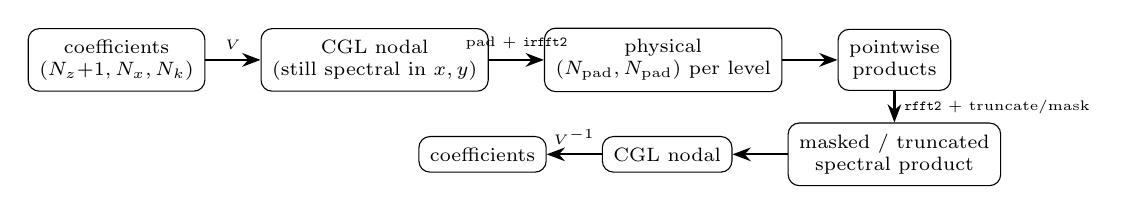
\begin{tikzpicture}[node distance=4mm and 7mm,
      box/.style={draw, rounded corners, align=center, inner sep=4pt, font=\scriptsize},
      arr/.style={-{Stealth}, thick}]
    \node[box] (c) {coefficients\\$(N_z{+}1,N_x,N_k)$};
    \node[box, right=of c] (n) {CGL nodal\\(still spectral in $x,y$)};
    \node[box, right=of n] (p) {physical\\$(N_{\rm pad},N_{\rm pad})$ per level};
    \node[box, right=of p] (m) {pointwise\\products};
    \node[box, below=of m] (b) {masked / truncated\\spectral product};
    \node[box, left=of b] (n2) {CGL nodal};
    \node[box, left=of n2] (c2) {coefficients};
    \draw[arr] (c) -- node[above,font=\tiny]{$V$} (n);
    \draw[arr] (n) -- node[above,font=\tiny]{pad + \texttt{irfft2}} (p);
    \draw[arr] (p) -- (m);
    \draw[arr] (m) -- node[right,font=\tiny]{\texttt{rfft2} + truncate/mask} (b);
    \draw[arr] (b) -- (n2);
    \draw[arr] (n2) -- node[above,font=\tiny]{$V^{-1}$} (c2);
  \end{tikzpicture}
  \end{center}
  \begin{itemize}
    \item Two advection forms, dispatched by \texttt{nonlinear\_advection}:
      Jacobian $\Jac{\psi}{f}$ or conservative flux $\nabla\!\cdot\!(\mathbf{u}f)$
      with $\mathbf{u}=(-\psi_y,\psi_x)$. \textbf{Production: flux.}
    \item Fused triple evaluation shares $\psi_x,\psi_y$ across
      $\Jac{\psi}{q'},\Jac{\psi}{w},\Jac{\psi}{\theta}$: 11 batched FFTs instead of 15.
    \item Note the arrow that matters for Part B: physical products re-enter spectral
      space through \texttt{rfft2} \emph{of a real array} --- so nonlinear
      tendencies are \textbf{exactly Hermitian}, always.
  \end{itemize}
\end{frame}

% ===========================================================================
\section{Dealiasing: the 3/2 and 2/3 rules}
% ===========================================================================

\begin{frame}{Aliasing in one slide}
  On an $N$-point periodic grid, wavenumbers are defined mod $N$: the pointwise
  product of modes $k_1,k_2$ contributes to $k_1+k_2$, and if $|k_1+k_2|>N/2$
  the contribution \emph{folds back} to $k_1+k_2\mp N$ --- an \textbf{alias image}
  landing on a resolved mode.
  \begin{itemize}
    \item For a quadratic nonlinearity with retained band $|k|\le K$, alias images
      land at $|k| \ge N - 2K$. They stay \emph{outside} the retained band iff
      \[
        N - 2K > K \quad\Longleftrightarrow\quad K < N/3 .
      \]
    \item Two classical implementations of the same math:
      \begin{enumerate}
        \item \textbf{3/2 rule}: keep all $N_x$ modes usable; evaluate products on a
          padded $\tfrac32 N_x$ grid so images fall in the padding, then truncate.
        \item \textbf{2/3 rule}: evaluate on the $N_x$ grid; zero all modes with
          $|k|>N_x/3$ after each product. Cheaper FFTs, fewer usable modes.
      \end{enumerate}
    \item On the shared band the two give bit-identical results --- the difference is
      where the FFT cost lives and how many stored modes carry physics.
  \end{itemize}
\end{frame}

\begin{frame}{The 3/2 rule (\texttt{32\_rule}; the historical default)}
  \begin{itemize}
    \item Pad $(N_x,N_k) \to (N_{\rm pad}, N_{\rm pad}/2{+}1)$ with
      $N_{\rm pad} = \tfrac32 N_x$; \texttt{irfft2}; multiply; \texttt{rfft2};
      truncate back.
    \item \textbf{Normalization bookkeeping} (a classic trap, done correctly here):
      zero-padding + \texttt{irfft2} attenuates physical values by
      $(N_x/N_{\rm pad})^2$; the product of two such fields by
      $(N_x/N_{\rm pad})^4$; converting the product back to $N_x$-grid DFT
      normalization contributes $(N_x/N_{\rm pad})^{-2}$; net correction
      $\boxed{(N_{\rm pad}/N_x)^2 = 9/4}$.
      Verified numerically to $10^{-13}$ during this review.
    \item Fine print: with $N_{\rm pad}=\tfrac32 N_x$ \emph{exactly}, products of
      $\pm N_x/2$ Nyquist pairs still self-alias onto the Nyquist shell (full safety
      needs $N_{\rm pad}\ge \tfrac32 N_x + 1$). Standard practice zeroes the Nyquist
      row/column; this code retains them. Normally invisible (dissipation kills
      Nyquist), but ``fully dealiased'' is not strictly true on that shell.
  \end{itemize}
\end{frame}

\begin{frame}{The 2/3 rule (\texttt{23\_rule}; production since April)}
  \begin{itemize}
    \item FFTs on the \emph{unpadded} $N_x$ grid; after each nonlinear product,
      multiply by a keep-mask
      $\;|k_x|\le K,\ k_y\le K$, $K = \lfloor N_x/3\rfloor$.
    \item Cost: FFT work drops by $\bigl(\tfrac{3}{2}\bigr)^2\times\frac{\log N_{\rm pad}}{\log N_x}
      \approx 2.4\times$ per product --- the motivation for switching
      (\file{efficiency\_review.md} \#6).
    \item Price: only $\sim(2N_x/3)^2$ of the stored $N_x^2$ modes carry physics.
      At fixed $N_x$ this is a genuine resolution change, not a free swap
      ($N_x{=}128$ under 2/3 $\approx$ $85^2$ usable modes).
  \end{itemize}
  \begin{alertblock}{Fine print found in this review (three items, all fixable cheaply)}
    \begin{enumerate}\small
      \item The mask is applied to product \emph{outputs only}; the \textbf{state is never
        truncated} --- and \texttt{make\_initial\_state} seeds noise on \emph{all} modes,
        restarts from 3/2-rule checkpoints import a populated top band. The alias-free
        guarantee assumes band-limited inputs; that invariant is unenforced.
      \item $K=\lfloor N_x/3\rfloor$ with ``$\le$'' is incompletely dealiased whenever
        $3\,|\,N_x$ (verified: $N_x{=}96$ leaves an $O(1)$ alias on the retained shell).
        $64/128/256$ are safe by accident; nothing guards it.
      \item At $N_x{=}64$: cutoff $k_{\rm cut}=21k_0\approx2.74$ sits \emph{inside} the
        instability band (edge $\approx3.16$) $\Rightarrow$ a linearly unstable,
        nonlinearly frozen band in the state. More in Part B context.
    \end{enumerate}
  \end{alertblock}
\end{frame}

% ===========================================================================
\section{Time integration: ARS(2,2,2) IMEX with unified dissipation}
% ===========================================================================

\begin{frame}{The IMEX splitting}
  \begin{center}
  \small
  \begin{tabular}{@{}lll@{}}
    \toprule
    equation & \textbf{explicit} $E(\cdot)$ & \textbf{implicit} $I(\cdot)$ \\
    \midrule
    $q'$ & $-\Jac{\psi}{q'} - i\beta k_x\hat\psi$ & $G_Z \hat w$ \quad (stretching) \\
    $w$ & $-\Jac{\psi}{w}$ & $c(k)\, G_Z \hat q' + \tfrac{\Rat}{\sigma}\hat\theta$ \\
    $\theta$ & $-\Jac{\psi}{\theta}\;[\,-\,w\,\dZ\Tb'\,]^{\dagger}$ & $\hat w$ \quad (conduction) \\
    $\Tb'$ & exchange substep$^{\dagger}$ & $\kappa_\theta G_{Z2}\Tb'$ \\
    \bottomrule
  \end{tabular}
  \end{center}
  {\footnotesize $c(k) = 1/(|k|^2+\Ld^{-2})$. $^{\dagger}$Under the production
  \texttt{balanced\_sbp2\_pc} branch the mean-exchange terms are \emph{removed} from the
  RHS and handled by a separate corrector (Sec.~5).}
  \begin{itemize}
    \item All horizontal dissipation is folded \emph{implicitly} into per-mode
      $\alpha$-factors (next slide) --- no explicit decay, no splitting error from
      stiff diffusion.
    \item The $w$--$\theta$ buoyancy coupling is implicit too: it has positive
      feedback at every $k$, so treating it explicitly would force tiny $\Delta t$.
  \end{itemize}
\end{frame}

\begin{frame}{ARS(2,2,2) and the unified dissipation factors}
  \begin{columns}[T]
    \column{0.52\textwidth}
    \begin{block}{Scheme ($\gamma = 1-\tfrac{1}{\sqrt2}$, $\delta = -\tfrac{\sqrt2}{2}$)}
      \small
      Stage 1 (implicit in $Y_1$):
      \[
        Y_1 = y^n + \gamma\Delta t\,\bigl(E(y^n) + I(Y_1)\bigr)
      \]
      Stage 2:
      \begin{align*}
        y^{n+1} = y^n + \Delta t\,\bigl[\,&\delta E(y^n) + (1{-}\delta)E(Y_1) \\
        &+ (1{-}\gamma) I(Y_1) + \gamma I(y^{n+1})\,\bigr]
      \end{align*}
      2nd order in both parts; L-stable implicit part.
      RK443 (Coral's ARS443 with correct final combination) is retained for
      comparison runs.
    \end{block}
    \column{0.46\textwidth}
    \begin{block}{Dissipation as $\alpha$-factors}
      \small
      \begin{align*}
        \alpha_q(k) &= 1 + \gamma\Delta t\,(\nu_q |k|^{2p} + \text{drag})\\
        \alpha_w(k) &= 1 + \gamma\Delta t\,\nu_w |k|^{2p}\\
        \alpha_\theta(k) &= 1 + \gamma\Delta t\,\tfrac{\nu_\theta}{\sigma}|k|^{2p}
      \end{align*}
      $p = \texttt{hyper\_order}$; production $p=1$ (Laplacian, Miquel-style),
      same $\nu=1$ on all fields.
      \par\smallskip
      \emph{Every one of these operators is diagonal in $(k_x,k_y)$ --- file that
      fact away for Part B.}
    \end{block}
  \end{columns}
\end{frame}

\begin{frame}{The implicit solve: block elimination per wavenumber}
  Per horizontal mode $k$, the stage system couples $\hat q',\hat w,\hat\theta$ in the
  vertical. Eliminate $\hat q'$ and $\hat\theta$ (both have diagonal-in-$Z$ solves):
  \[
    \hat q' = \frac{r_q + \gamma\Delta t\, G_Z\hat w}{\alpha_q},
    \qquad
    \hat\theta = \frac{r_\theta + \gamma\Delta t\, \hat w}{\alpha_\theta},
  \]
  and substitute into the $w$ row to get one dense vertical solve:
  \[
    \underbrace{\Bigl[\alpha_{w,\mathrm{eff}}\, \mathbb{I}
      \;-\; (\gamma\Delta t)^2\, c(k)\, B\Bigr]}_{A'(k)} \hat w = \mathrm{rhs},
    \qquad
    \alpha_{w,\mathrm{eff}} = \alpha_w - \frac{(\gamma\Delta t)^2\,\Rat/\sigma}{\alpha_\theta},
  \]
  where $B = P^{\dashv} G_Z\, \alpha_q^{-1} G_Z\, S$ is assembled in the reduced
  Dirichlet--Galerkin space ($S$ = stencil, $P^{\dashv}$ = exact left inverse).
  \begin{itemize}
    \item $(A')^{-1}$ is \textbf{precomputed} per mode and applied as a matmul ---
      JAX-friendly (no per-step LU). Conditioning is benign:
      measured $\mathrm{cond}(A') \in [1.0, 2.9]$ at production $\Delta t$
      (the $(\gamma\Delta t)^2$ prefactor keeps the stiff block tiny).
    \item Back-substitute $\hat q'$, $\hat\theta$; solve the $\Tb'$ tau system.
  \end{itemize}
\end{frame}

\begin{frame}{Shell deduplication and the JAX execution model}
  \begin{itemize}
    \item $A'(k)$ depends on $k$ only through $|k|^2$ $\Rightarrow$ store one inverse
      per distinct $|k|^2$ \emph{shell}: $5924$ shells at $N_x{=}256$ vs
      $\sim3.3\times10^4$ modes; $\sim8.3\times10^4$ shells at $N_x{=}1024$.
    \item Caveats found in review:
      (i) for \texttt{q\_boundary='none'} the $q$-solve is stored as dense scaled
      \emph{identities} per shell while the scalar $1/\alpha_q$ that would replace
      them sits precomputed and unused;
      (ii) at run time the gather \texttt{mat\_shells[ksq\_idx]} materializes the
      full $(N_x,N_k,N_z{+}1,N_z{+}1)$ tensor ($\sim$1.1\,GB per gather at
      $64{\times}256$) --- the root of the recorded 114\,GB peak;
      (iii) the whole grid is \emph{captured as jit constants}
      ($\sim$14\,GB at $256^2{\times}384$).
  \end{itemize}
  \begin{block}{Measured V100 float64 baseline (\file{CLAUDE.md} benchmark)}
    \scriptsize
    \begin{tabular}{@{}rrrrrr@{}}
      \toprule
      $N_x$ & $N_z$ & ms/step & steps/s & state MB & shells \\
      \midrule
      128 & 16 & 2.9 & 347 & 6.8 & 1621 \\
      256 & 32 & 24.2 & 41 & 52 & 5924 \\
      1024 & 64 & 967 & 1.0 & 1639 & 82817 \\
      \bottomrule
    \end{tabular}
    \quad\parbox[b]{0.42\textwidth}{\scriptsize Production loop: Python \texttt{for} around
    \texttt{jax.jit(step)} with \texttt{donate\_argnums}; dispatch overhead
    $<0.1\%$ at production sizes. Keep BLAS threads at 1 during grid build
    (host-side dense inverses, not XLA, cause the startup stall).}
  \end{block}
\end{frame}

% ===========================================================================
\section{The mean--fluctuation thermal exchange}
% ===========================================================================

\begin{frame}{Why the exchange pair is delicate}
  The two exchange terms are energetic mirror images. Multiply the $\theta$ equation
  by $\theta$ and average; multiply the $\Tb'$ equation by $\Tb'/\mu$ and integrate:
  \[
    \frac{d}{dt}\frac{\|\theta\|^2}{2}\;\supset\; -\int \dZ\Tb'\,\avexy{w\theta}\,dZ,
    \qquad
    \frac{d}{dt}\frac{\|\Tb'\|^2}{2\mu}\;\supset\; -\int \Tb'\,\dZ\avexy{w\theta}\,dZ .
  \]
  Integrating by parts (boundary terms vanish under the Dirichlet BCs), the two are
  \emph{equal and opposite}: the exchange moves variance between reservoirs without
  creating any.
  \begin{alertblock}{The discrete requirement}
    The semi-discrete versions of $-w\,\dZ\Tb'$ and $-\mu\,\dZ\avexy{w\theta}$ must be
    \textbf{negative adjoints of one bilinear form under the chosen discrete inner
    products} --- otherwise the pair pumps or leaks variance, invisibly, at every step.
    The naive CGL/Clenshaw--Curtis construction is \emph{not} such an adjoint pair.
  \end{alertblock}
  This single requirement drove the entire branch sequence of March--April.
\end{frame}

\begin{frame}{Branch history at a glance ($64^2\times256$, $\Delta t = 5\times10^{-5}$)}
  \begin{center}
  \small
  \begin{tabular}{@{}lll@{}}
    \toprule
    branch & idea & outcome \\
    \midrule
    \texttt{legacy} & naive CGL exchange & non-finite at $t=11.22$ \\
    \texttt{coral\_workgrid\_flux} & shared work-grid products & $t=11.44$ \\
    \texttt{coral\_workgrid\_weakmean/paired} & adjoint-flavored & worse; retired \\
    \texttt{balanced\_midpoint} & frozen-$w$ CN on Chebyshev & unstable $t\approx10.4$--$10.6$ \\
    \texttt{balanced\_sbp2} & frozen-$w$ CN on uniform SBP grid & delayed failure $t=41.05$ \\
    \texttt{balanced\_sbp2\_pc} + sub4 & stage-wise predictor--corrector & \textbf{clean: $t=80$, then $t=120$} \\
    \bottomrule
  \end{tabular}
  \end{center}
  \begin{itemize}
    \item Two meta-lessons recorded in \file{adjoint\_mean\_exchange.md}:
      (i) a shared product-build path helps; abstract ``adjointness'' alone does not;
      (ii) \emph{restart timing is part of the experiment} --- late branch-switch
      restarts inherit contaminated states and slander good branches
      (the $t{=}42$ vs $t{=}40$ restart comparison).
    \item Part B adds a third lesson: some of the ``contamination'' being inherited
      was not physical at all.
  \end{itemize}
\end{frame}

\begin{frame}{\texttt{balanced\_sbp2\_pc}: the production scheme}
  \textbf{Idea: decouple the exchange algebra from the IMEX coupling.}
  Per ARS222 stage:
  \begin{enumerate}
    \item \textbf{Predictor}: run the base ARS222 stage \emph{without} exchange
      (fixed-conduction RHS).
    \item \textbf{Corrector}: apply a frozen-$w$ balanced thermal substep
      $P_\alpha$ (next slide) to the stage state, over the stage interval
      $\gamma\Delta t$, optionally subcycled (\texttt{sbp\_corrector\_substeps=4}
      in production $\Rightarrow$ 8 substeps per timestep).
    \item The stage-1 correction tendency $C_1 = (P_\alpha Y_1 - Y_1)/(\gamma\Delta t)$
      re-enters the stage-2 explicit combination with weight $(1-\gamma)\Delta t$
      --- the implicit column still sums to $\Delta t$; the scheme stays 2nd order.
  \end{enumerate}
  \begin{itemize}
    \item Verified during review: tableau weights consistent; the hoisted
      implementation (invariants of the substep loop precomputed once per stage)
      is bit-identical to the reference and saves $\sim$18 padded FFTs/step.
    \item FFT budget note: at sub4 the corrector does \emph{more} FFT work than the
      nonlinear advection ($\sim$32 of $\sim$54 padded FFTs/step).
  \end{itemize}
\end{frame}

\begin{frame}{Inside the corrector: frozen-$w$ midpoint solve on a uniform SBP grid}
  Uniform grid $z_j = j/N$, second-order SBP operators: diagonal norm $H$,
  first derivative $D_1$ (exact SBP property $HD_1 + D_1^{\!\top}H = \mathrm{diag}(-1,0,\dots,0,1)$,
  verified), Laplacian $L$. With $w^\star$ frozen, per substep:
  \[
    F_n(z) = \avexy{w^\star \theta_n}, \qquad
    M = \mathrm{diag}\,\avexy{(w^\star)^2},
  \]
  \[
    A\,\Tb_{n+1} = B\,\Tb_n - \mu\Delta t\, D_1 F_n,
    \qquad
    A/B = \mathbb{I} \mp \tfrac12\mu\kappa_\theta\Delta t\, L
      \mp \tfrac14 \mu \Delta t^2\, D_1 M D_1,
  \]
  then update fluctuations with the \emph{midpoint} gradient
  $g_{n+1/2} = \tfrac12 D_1(\Tb_n + \Tb_{n+1})$:
  \(
    \;\theta_{n+1} = \theta_n - \Delta t\, w^\star\, g_{n+1/2}.
  \)
  \begin{itemize}
    \item By construction the pair cancels in the SBP norm: the discrete exchange
      residual on the SBP grid is a \emph{boundary term}, which the Dirichlet rows
      kill $\Rightarrow$ $R_{\rm ex}^{\rm sbp}$ sits at roundoff for the entire
      $t=120$ run.
    \item The horizontal averages $\avexy{\cdot}$ use the same dealiased product path
      as everything else (padded grid under 3/2; $N_x$ grid under 2/3, where the
      mean of a band-limited product is alias-free by Parseval).
  \end{itemize}
\end{frame}

\begin{frame}{The transfer layer: CGL $\leftrightarrow$ uniform SBP}
  The corrector lives on a uniform grid; the solver on CGL. Why not evaluate
  Chebyshev coefficients directly on the uniform grid? Because the
  Chebyshev-on-uniform Vandermonde is \emph{catastrophically ill-conditioned} by
  $N_z=256$. The implemented choice (\texttt{sbp\_transfer\_mode='interp'}):
  \textbf{piecewise-linear} interpolation matrices both ways.
  \begin{alertblock}{Review finding: this is also an uncontrolled near-wall filter}
    \begin{itemize}\small
      \item CGL nodes cluster as $Z_1 \approx (\pi/N_z)^2/4$: at $N_z{=}256$,
        \textbf{11 CGL points sit inside the first uniform cell}. Every corrector
        substep replaces their $\theta$ values with a 2-point linear interpolant ---
        applied $8\times$ per step, $\sim1.6\times10^5$ times per time unit.
      \item Measured: roundtrip $R\,T$ has $\max|RT-\mathbb{I}| = 1.0$ at the first
        interior CGL node; spectral radius exactly 1 (non-amplifying --- stable),
        $\sin(\pi Z)$ roundtrip error $4\times10^{-5}$ per application at $N_z{=}256$.
      \item Consequences: (i) some of \texttt{balanced\_sbp2\_pc}'s robustness may be
        this implicit smoothing rather than the balanced algebra;
        (ii) $\theta$'s vertical accuracy near the walls is capped at 2nd order;
        (iii) the thermal boundary layer --- \emph{which sets Nu} --- is filtered.
        Prime suspect for the Nu gap (Sec.~7).
    \end{itemize}
  \end{alertblock}
\end{frame}

\begin{frame}{Current best runs (the ``stable runs'' of Part B)}
  \begin{center}
  \small
  \begin{tabular}{@{}lllll@{}}
    \toprule
    run & reached & $\Nud$ & $R_{\rm ex}^{\rm sbp}$ & notes \\
    \midrule
    $64^2\times256$, from $t{=}20$ & $t=80$ & $19.5$ & $0.0$ & first clean crossing of the $t\approx50$ window \\
    $128^2\times256$ chain & $\mathbf{t=120}$ & $19$--$22$ & $\le 2{\times}10^{-15}$ & upsampled from $64^2$ at $t{=}40$; 2/3-rule \\
    $256^2\times256$ chain & $t=63$ & $16$--$18$ & $0.0$ & 2/3-rule \\
    \bottomrule
  \end{tabular}
  \end{center}
  \begin{itemize}
    \item All: \texttt{balanced\_sbp2\_pc}, sub4, flux advection, $\Delta t = 5\times10^{-5}$,
      $\Rat=100$, float64. Fields bounded and sane: $\max|w| \sim 200$--$420$,
      $\max|\theta| \sim 5$--$18$, $KE_{\rm bt}\sim(2.5$--$4.5){\times}10^3$.
    \item So: the late-time state failure that consumed March--April is
      \textbf{operationally solved}.
    \item And yet, in these same clean runs, the \emph{raw} thermal diagnostics
      read $\Nuraw \sim 10^{27}$ and $KE_{\rm bc}\sim10^{28}$ at $t=120$.
      Explaining that is Part B.
  \end{itemize}
\end{frame}

% ===========================================================================
\section[Part B: aliased vs dealiased, diagnosed]{Part B --- The aliased-vs-dealiased ``blowup'' of the stable runs, diagnosed}
% ===========================================================================

\begin{frame}{Two ways to measure the same heat flux}
  For \texttt{thermal\_closure='evolve\_mean'} the archives carry two Nusselt numbers:
  \begin{columns}[T]
    \column{0.5\textwidth}
    \begin{block}{Raw (``aliased'') $\Nuraw$}
      \small
      Parseval-style inner product of the stored spectral coefficients:
      \[
        \avexy{w\theta}(Z_j) = \frac{1}{N_x^4}\sum_{k}\mathrm{Re}\,
          \hat w\,\hat\theta^{*}\cdot \varpi_k
      \]
      ($\varpi_k$ = rfft half-plane weights), then CC quadrature in $Z$.
      \emph{Never leaves spectral space.}
    \end{block}
    \column{0.48\textwidth}
    \begin{block}{Dealiased $\Nud$}
      \small
      The same product path the mean equation uses: transform to the
      (padded) physical grid via \texttt{irfft2}, multiply pointwise,
      average, CC quadrature.
      \emph{Passes through a real physical field.}
    \end{block}
  \end{columns}
  \medskip
  For coefficients that represent a genuine real field, the two agree up to small
  Nyquist-band correlation differences. The operational doctrine since April:
  \emph{trust $\Nud$, keep $\Nuraw$ as an ``aliased comparison metric''.}
  That doctrine was right --- but the accepted mechanism (``aliasing noise'') was not.
\end{frame}

\begin{frame}{What the stable runs actually record}
  \begin{center}
  \small
  \begin{tabular}{@{}llrrl@{}}
    \toprule
    run & $t$ & $\Nuraw$ & $\Nud$ & other \\
    \midrule
    $128^2{\times}128$ (t8-era archive) & 8.0 & $1.68\times10^{17}$ & $38.9$ & \\
    $64^2{\times}256$ (t8-era archive) & 8.0 & $5.12\times10^{18}$ & $37.0$ & \\
    \midrule
    $128^2{\times}256$ chain & 40.0 & $15.5$ & $15.5$ & \textbf{clean at restart} \\
     & 74.0 & $1.5\times10^{15}$ & $14.8$ & $KE_{\rm bc}=7.9\times10^{15}$ \\
     & 120.0 & $6.6\times10^{27}$ & $21.9$ & $KE_{\rm bc}=9.1\times10^{28}$ \\
    \midrule
    $256^2{\times}256$ chain & 63.0 & $6.5\times10^{3}$ & $15.8$ & younger contamination \\
    \bottomrule
  \end{tabular}
  \end{center}
  \begin{itemize}
    \item The raw diagnostics grow \emph{smoothly and exponentially} for 80 time units
      while every physical-space observable stays flat:
      at $t{=}120$: $\max|\mathbf{u}| = 488$, $\max|w| = 412$, $\max|\theta| = 18.2$,
      $KE_{\rm bt} = 4.0\times10^{3}$.
    \item Note the restart at $t{=}40$ (from a Fourier-upsampled checkpoint) begins
      with $\Nuraw = \Nud$ \emph{exactly} --- whatever grows was reset by upsampling.
  \end{itemize}
\end{frame}

\begin{frame}{Step 1 of the diagnosis: the numbers are mutually impossible}
  Both diagnostics are computed \textbf{from the same arrays} $\hat w,\hat\theta$.
  If those arrays represent real fields $w(x,y),\theta(x,y)$ on the grid, then
  Parseval's identity makes the raw diagnostic the \emph{exact} grid mean of the
  pointwise product, so
  \[
    \bigl|\avexy{w\theta}\bigr| \;\le\; \max|w|\cdot\max|\theta|
    \;\approx\; 412 \times 18.2 \;\approx\; 7.5\times10^{3}.
  \]
  But the recorded raw value at $t{=}120$ is
  \[
    \texttt{tw\_raw} \;=\; 6.6\times10^{27}.
  \]
  \begin{alertblock}{Conclusion (no code inspection needed)}
    The stored coefficients \textbf{cannot represent any real field}. Since
    $\max|w|$ comes from \texttt{irfft2} of the \emph{same} array, the excess must
    live in components that \texttt{irfft2} silently discards --- i.e.\ the state
    violates the reality (Hermitian-symmetry) constraints of the \texttt{rfft2}
    layout.
  \end{alertblock}
  This also rules out the old reading: classical aliasing redistributes the energy
  of a \emph{real} field --- it can never break the Parseval bound.
\end{frame}

\begin{frame}{Step 2: where reality constraints live in an \texttt{rfft2} array}
  An $(N_x,\ N_x/2{+}1)$ \texttt{rfft2} array represents a real field iff its
  self-conjugate columns satisfy pairing in $k_x$:
  \[
    \hat f(-k_x,\,k_y{=}0) = \hat f(k_x,\,k_y{=}0)^{*},
    \qquad\text{(and the same at } k_y = N_x/2\text{)} .
  \]
  Decompose those columns into Hermitian + anti-Hermitian parts:
  \[
    \hat f_{\pm}(k_x) = \tfrac12\bigl(\hat f(k_x) \pm \hat f(-k_x)^{*}\bigr).
  \]
  \begin{itemize}
    \item \texttt{irfft2} reconstructs the physical field from $\hat f_{+}$ only:
      the anti-Hermitian part $\hat f_{-}$ contributes \emph{nothing} to any
      physical-space evaluation. (Verified empirically: an
      \texttt{irfft2}$\to$\texttt{rfft2} roundtrip removes it.)
    \item Quadratic spectral sums --- $\Nuraw$, $KE$, rms values, shell budgets ---
      count $|\hat f_{+}|^2 + |\hat f_{-}|^2$. They see it all.
  \end{itemize}
  \begin{block}{So the question becomes}
    Is there anti-Hermitian content in the state? How big, where, and why growing?
  \end{block}
\end{frame}

\begin{frame}{Step 3: measure it on the checkpoints (this review, verified directly)}
  \begin{center}
  \small
  \begin{tabular}{@{}llrrr@{}}
    \toprule
    checkpoint & field & $\max|\hat f_{+}|$ ($k_y{=}0$) & $\max|\hat f_{-}|$ ($k_y{=}0$) &
      $\dfrac{E_{\rm Parseval}}{E_{\rm projected}}$ \\
    \midrule
    $t{=}120$, $128^2{\times}256$ & $q'$ & $\sim10^{5}$ & $1.07\times10^{19}$ & $5.9\times10^{26}$ \\
     & $w$ & & $2.85\times10^{18}$ & $6.8\times10^{24}$ \\
     & $\theta$ & & $1.43\times10^{17}$ & $1.1\times10^{26}$ \\
    \midrule
    $t{=}8$, $64^2{\times}256$ (old archive) & $q'$ & $8.8\times10^{3}$ & $2.26\times10^{13}$ & $3.4\times10^{16}$ \\
    \bottomrule
  \end{tabular}
  \end{center}
  \begin{itemize}
    \item The $k_y{=}0$ column is \emph{pure ghost}: the measured violation equals
      $2\max|\hat f|$ to the digit, i.e.\ $\hat f(k_x,0) \simeq -\hat f(-k_x,0)^{*}$
      --- anti-Hermitian to all displayed digits.
    \item The $k_y$-Nyquist column is exactly zero (dissipation keeps it clean).
    \item Projected (physical) energies are perfectly moderate --- the resolved
      solution underneath is healthy, exactly as $\Nud$ said.
  \end{itemize}
\end{frame}

\begin{frame}{Step 4: why it grows --- a linear instability with the saturation removed}
  \begin{center}
  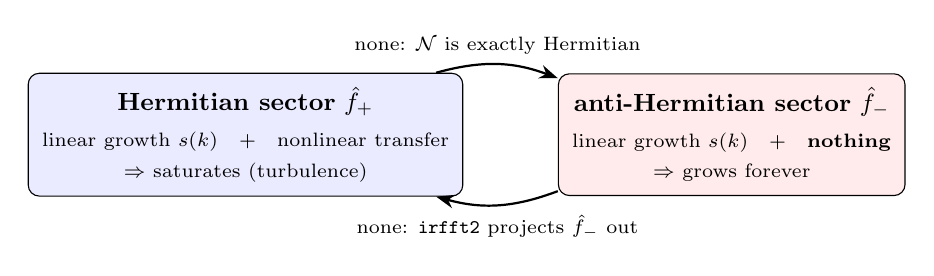
\begin{tikzpicture}[node distance=4mm and 12mm,
      box/.style={draw, rounded corners, align=center, inner sep=5pt, font=\small},
      arr/.style={-{Stealth}, thick}]
    \node[box, fill=blue!8] (phys) {\textbf{Hermitian sector} $\hat f_{+}$\\[2pt]
      \scriptsize linear growth $s(k)$ \; + \; nonlinear transfer\\
      \scriptsize $\Rightarrow$ saturates (turbulence)};
    \node[box, fill=red!8, right=of phys] (ghost) {\textbf{anti-Hermitian sector} $\hat f_{-}$\\[2pt]
      \scriptsize linear growth $s(k)$ \; + \; \textbf{nothing}\\
      \scriptsize $\Rightarrow$ grows forever};
    \draw[arr] (phys) to[bend left=18] node[above,font=\scriptsize]{none: $\mathcal{N}$ is exactly Hermitian} (ghost);
    \draw[arr] (ghost) to[bend left=18] node[below,font=\scriptsize]{none: \texttt{irfft2} projects $\hat f_{-}$ out} (phys);
  \end{tikzpicture}
  \end{center}
  \begin{enumerate}
    \item Nonlinear tendencies are \texttt{rfft2} of \emph{real} pointwise products
      $\Rightarrow$ \textbf{exactly Hermitian} $\Rightarrow$ they feed the ghost nothing,
      and the ghost (invisible to \texttt{irfft2}) feeds nothing back.
    \item Every linear operation --- $\psi$ inversion, $\alpha$-factors, the per-shell
      implicit solve, stretching, buoyancy, conduction --- is \textbf{diagonal in
      $(k_x,k_y)$} and Hermitian-blind: it evolves $\hat f_{-}$ with the same
      linearized dynamics as a physical mode.
    \item Result: the anti-Hermitian sector of the $k_y{=}0$ column integrates the
      \emph{linearized} NHQG system with \textbf{no eddy saturation}: pure exponential
      growth from a roundoff seed, forever.
  \end{enumerate}
\end{frame}

\begin{frame}{Step 5: quantitative closure --- the growth rates match linear theory}
  \begin{itemize}
    \item \textbf{Early (fresh run, conduction-state gradients).}
      Old $t{=}8$ archive: ghost amplitude $2.26\times10^{13}$ from a roundoff seed
      $\sim10^{-16}$ gives
      \[
        s_{\rm ghost} = \frac{\ln(2.26\times10^{13}/10^{-16})}{8} \approx 8.4
        \quad\text{vs.}\quad
        s_{\max} \approx 8.6 \ \text{at } k\approx0.83 .
      \]
    \item \textbf{Late (saturated mean state).} $128^2{\times}256$ chain:
      ghost energy $\sim10^{3}\to 9.1\times10^{28}$ over $t=40\to120$
      $\Rightarrow$ amplitude rate $\approx 0.37$/unit --- the \emph{residual}
      growth rate of the marginal mode on the turbulently flattened mean gradient.
      (This is why the raw diagnostics of the stable runs grow gently for 80 units
      instead of exploding in 8.)
    \item \textbf{Location.} The ghost concentrates at $k_y{=}0$,
      $|k_x| \approx 0.9$--$1.0$ --- the fastest-growing linear modes that fit the
      box.
  \end{itemize}
  \begin{alertblock}{Full consistency}
    Impossibility bound + direct measurement + mechanism + two independent
    growth-rate checks. The ``raw blowup'' of the stable runs is a
    \textbf{non-Hermitian ghost mode}, not physics and not classical aliasing.
  \end{alertblock}
\end{frame}

\begin{frame}{Step 6: the ghost fooled more than the Nusselt number}
  \begin{columns}[T]
    \column{0.55\textwidth}
    \begin{alertblock}{The $k\approx0.9786$ ``dominant shell''}
      The April spectral campaign concluded: \emph{``the dominant positive KE source
      is low-shell stretching near $k\approx0.9786$.''} But
      \texttt{ke\_stretch\_shell\_tendency} is a spectral inner product
      (ghost-visible), and $k\approx0.98$ \textbf{is the ghost's home shell}
      ($k_y{=}0$, $k_x\approx7.5\,k_0$; bin-center label). The dominant-shell
      story, the exploding \texttt{th\_mean\_feedback\_sum} ($\sim-10^{16}$), and the
      ``low-shell source chain'' need re-derivation from Hermitian-projected states
      before any physics is read from them.
    \end{alertblock}
    \column{0.43\textwidth}
    \begin{block}{Archive triage}
      \footnotesize
      \textbf{Ghost-visible (spectral sums):}\\
      \texttt{Nusselt}, \texttt{vol\_avg\_tw}, $KE_{\rm bc}$/$KE_{\rm tot}$,
      \texttt{ke\_*\_shell\_tendency}, \texttt{ke\_nonlinear\_flux},
      \texttt{q/w/th\_horiz\_spec}, \texttt{*\_rms},
      \texttt{vertical\_mode\_energy}, \texttt{th\_mean\_feedback\_sum},
      \texttt{heat\_flux\_mismatch}.
      \par\smallskip
      \textbf{Ghost-blind (physical products):}\\
      \texttt{Nusselt\_dealiased}, \texttt{vol\_avg\_tw\_dealiased},
      dealiased shell budgets and exchange residuals,
      \texttt{max\_w/max\_theta/max\_speed}, $\Tb'$ profiles,
      $R_{\rm ex}^{\rm sbp}$.
    \end{block}
  \end{columns}
  \medskip
  \small The doctrine ``trust the dealiased diagnostics'' was correct ---
  they are ghost-blind \emph{because} they pass through \texttt{irfft2}.
  The label ``aliased'' for the raw ones was a misnomer: genuine aliasing
  (Nyquist-band correlations) is a small, bounded effect here.
\end{frame}

\begin{frame}{Step 7: seeding, and two accomplices}
  \begin{itemize}
    \item \textbf{Seed 1 (always present):} FFT roundoff. \texttt{rfft2} of a real
      array is Hermitian only to machine precision $\Rightarrow$ every step deposits
      $O(10^{-16})$ anti-Hermitian dust, which the linear dynamics then amplify.
    \item \textbf{Seed 2 (avoidable):} \texttt{make\_initial\_state}
      (\file{solver.py:1224}) draws \emph{independent complex noise on all modes} ---
      it violates Hermitian symmetry at $t=0$ by construction, at the full noise
      amplitude.
    \item \textbf{Accomplice 1:} the 2/3-rule state is never truncated (Sec.~3
      fine print) --- an adjacent ``unsaturated sector'' issue: at $N_x{=}64$ the
      masked band $k\in(2.74,3.16)$ is linearly unstable with the nonlinear transfer
      masked away; it can only saturate quasilinearly by flattening $\Tb'$.
    \item \textbf{Accomplice 2:} the FD benchmark (\file{fd\_vertical\_benchmark/})
      has the identical disease, independently: raw Nu $\sim10^{29\text{--}31}$ with
      $\max|w|\max|\theta| \sim 5.7\times10^{4}$, and \emph{its} SBP residual
      ($-3.4\times10^{29}$ at $t{=}10$) is computed spectrally $\Rightarrow$
      currently meaningless late in a run. No Hermitian enforcement exists anywhere
      in that package either.
  \end{itemize}
\end{frame}

\begin{frame}{The fix: one projection, three lines of intent}
  \begin{block}{1. Symmetrize the self-conjugate columns after each step (or every $K$ steps)}
    For each evolved field, on the $k_y{=}0$ column (and $k_y$-Nyquist if retained):
    \[
      \hat f(k_x, 0) \;\leftarrow\; \tfrac12\Bigl(\hat f(k_x,0) + \hat f(-k_x,0)^{*}\Bigr)
    \]
    \footnotesize In JAX: \texttt{f.at[:, :, 0].set(0.5*(f[:, :, 0] + jnp.conj(f[:, neg\_ix, 0])))}
    with \texttt{neg\_ix = (-jnp.arange(Nx)) \% Nx}. Cost: negligible (one
    $(N_z,N_x)$ slice per field). Per-step ghost growth is
    $e^{8.6\cdot 5\times10^{-5}} \approx 1.0004$, so even every-100-steps projection
    holds the ghost at $\sim10^{-14}$.
  \end{block}
  \begin{block}{2. Fix the seed and guard the invariant}
    Make \texttt{make\_initial\_state} Hermitian (draw real noise, \texttt{rfft2} it);
    add a regression test: step $N$ times, assert the anti-Hermitian norm of each
    field stays at roundoff.
  \end{block}
  \begin{block}{3. Re-derive the contaminated conclusions}
    Re-run \file{scripts/analyze\_dominant\_shell.py} and the KE shell budgets on
    Hermitian-projected checkpoints; port the projection into \file{fd\_vertical\_benchmark/}.
  \end{block}
\end{frame}

\begin{frame}{Bonus: raw $\approx$ dealiased becomes a free integrity audit}
  Once the state is Hermitian-projected \emph{and} (under 2/3) band-limited:
  \begin{itemize}
    \item $\Nuraw$ and $\Nud$ should agree to near machine precision --- for a
      band-limited product on the $N_x$ grid, the horizontal \emph{mean} is exactly
      alias-free (any alias image into $k{=}0$ would need $|k_1+k_2| = N_x$,
      impossible with $|k_i|\le N_x/3$).
    \item So the cheap raw diagnostic stops being a ``known-bad comparison metric''
      and becomes a \textbf{continuous consistency check}: any re-divergence of
      $\Nuraw$ from $\Nud$ flags a new leak (mask hole, symmetry break, transfer bug)
      the moment it appears, instead of $10^{27}$ later.
    \item Same for $KE_{\rm bc}$ vs physical-space KE, and for the FD benchmark's
      residual.
  \end{itemize}
  \medskip
  \emph{The March motif closes: the $D_Z$ null mode, the frozen 2/3 band, and the
  anti-Hermitian ghost are all the same disease --- state components outside the
  representation the physics actually sees, amplified by linear dynamics. The cure
  is always the same: make the invariant explicit and project onto it.}
\end{frame}

% ===========================================================================
\section{Revised audit hierarchy and open issues}
% ===========================================================================

\begin{frame}{What each audit can and cannot see (revised)}
  \begin{center}
  \small
  \begin{tabular}{@{}lll@{}}
    \toprule
    audit & sees & blind to \\
    \midrule
    $R_{\rm ex}^{\rm sbp}$ ($\equiv0$) & SBP operator algebra & \emph{everything else}$^{\dagger}$ \\
    $R_{\rm ex}^{d}$ (dealiased residual) & exchange closure on CGL side & attributes transfer error to ``exchange'' \\
    $\Nuraw$ vs $\Nud$ (post-fix) & symmetry/band leaks & vertical-transfer smoothing \\
    anti-Hermitian norm (new) & ghost content directly & --- \\
    \bottomrule
  \end{tabular}
  \end{center}
  {\footnotesize $^{\dagger}$Review finding: $R_{\rm ex}^{\rm sbp}$ reduces to
  $\Tb^{\top}(HD_1 + D_1^{\top}H)F = $ boundary term, which the Dirichlet BCs kill
  \emph{identically} --- it is a structural identity of the operators, not a
  time-step audit. It would read $0.0$ even with a wrong exchange coefficient or
  sign. \file{CLAUDE.md}'s ``the trusted exchange audit is now the SBP-side
  residual'' overstates it.}
  \begin{itemize}
    \item Also in the diagnostics fine print: under \texttt{balanced\_sbp2\_pc} the
      archived \texttt{th\_nonlinear/th\_total} shell decomposition subtracts a
      mean-feedback term the RHS never contained (mislabeled, non-conservative);
      \texttt{q/w/th\_horiz\_spec} lack the $N_x^4$ normalization that
      \texttt{ke\_horiz\_spec} has (cross-resolution comparisons off by
      $(N_{x,1}/N_{x,2})^4$).
  \end{itemize}
\end{frame}

\begin{frame}{The now-headline open problem: the Nusselt gap}
  \begin{center}
    $\Nud \approx 18$--$20$ (time-mean, stable runs, $\Rat=100$)
    \quad vs.\quad
    Miquel: $43.37 \pm 2.54$.
  \end{center}
  Stability is solved; \textbf{accuracy is not}. Candidate causes, in suspected order:
  \begin{enumerate}
    \item \textbf{Near-wall transfer smoothing} (Sec.~5): the piecewise-linear
      CGL$\leftrightarrow$SBP roundtrip filters the thermal boundary layer
      $8\times$/step --- and Nu \emph{is} the boundary-layer gradient.
      Test: A/B \texttt{sbp\_corrector\_substeps} 4 vs 1, and \texttt{interp} vs a
      higher-order/mass-consistent transfer, watching $\Nud$ + near-wall
      $\theta$ spectra.
    \item \textbf{$N_x{=}64$ heritage}: the $128^2$ chain was upsampled from a
      $64^2$ state whose masked band could only saturate by flattening
      $\Tb'$ (Sec.~3 fine print); a flattened mean suppresses heat flux.
      Test: long fresh $128^2$ run after the state-masking fix.
    \item \textbf{Effective resolution under 2/3}: $128^2$ stored $\to$ $85^2$
      usable vs Miquel's fully-usable $256^2$ at $\Rat{=}100$
      (their Nu is resolution-sensitive: they moved to $256^2{\times}384$ for it).
    \item Residual formulation differences (worth ruling out only after 1--3).
  \end{enumerate}
\end{frame}

\begin{frame}{Side campaign: FD-vertical (toward asymmetric BCs)}
  Goal: eventual \textbf{Neumann-$w$ top / Dirichlet bottom} (Jupiter-relevant), which
  Chebyshev-tau handles awkwardly $\Rightarrow$ SBP-SAT finite differences in the
  vertical. Status after May 29 ($64^2{\times}256$ probes):
  \begin{itemize}
    \item \textbf{Operator family exonerated}: \texttt{compact4} and \texttt{sbp42}
      fail identically at $t\approx4$ --- the culprit was a spurious
      $\psi$-Neumann boundary treatment, the FD re-run of the March
      \texttt{q\_boundary='none'} lesson.
    \item With \texttt{psi\_boundary='none'}: uniform grid dies at $t\approx9.4$;
      \textbf{tanh-stretched grid ($\beta{=}4$) ran finite to $t=10$} with bounded
      fields --- first end-to-end FD-vertical survival of the historical danger window.
    \item Not yet done: any actual SAT mixed-BC run (the reason SBP was chosen);
      Nu validation (blocked by the same ghost bug in its diagnostics --- port the
      projection); corrector subcycling is inert there (sub1 $\equiv$ sub4 to 4
      digits).
  \end{itemize}
\end{frame}

\begin{frame}{Prioritized action list}
  \begin{enumerate}
    \item \textbf{Commit the repository.} It has \emph{zero git commits} --- solver,
      tests, and all notes exist only as working-tree files.
      \texttt{.gitignore} for \file{output/} (310\,GB), logs, PDFs; then commit.
    \item \textbf{Hermitian projection} + Hermitian initial noise + anti-Hermitian-norm
      regression test; re-run dominant-shell/KE-budget analyses on projected
      checkpoints; port to \file{fd\_vertical\_benchmark/}.
    \item \textbf{Mask the 2/3-rule state} at init/restart/finalize; add an
      $N_x \bmod 3 \ne 0$ guard.
    \item \textbf{Attack the Nu gap} via the transfer-layer experiments (previous
      slide) --- this is now the science-critical question.
    \item \textbf{Driver hygiene}: store the config dict inside checkpoints
      (restart physics currently depends on retyping CLI flags whose silent defaults
      are \texttt{legacy}/\texttt{32\_rule}/\texttt{jacobian}); non-finite early
      stop (May 29 runs burned $\sim$60\% of GPU time stepping NaN); incremental
      archive writes; run-name uniqueness.
    \item \textbf{Refresh the docs}: \file{CLAUDE.md} status sections (two
      generations stale), test counts (89, not 50), state-layout section,
      \file{experiments.md} Miquel table, \texttt{float\_dtype} default
      (\texttt{"float32"} in code vs documented float64).
  \end{enumerate}
\end{frame}

\begin{frame}{Map: where everything lives}
  \footnotesize
  \begin{columns}[T]
    \column{0.5\textwidth}
    \textbf{Code}
    \begin{itemize}\itemsep1pt
      \item \file{nhqg/config.py} --- \texttt{NHQGConfig} (beware: bare defaults
        match production on almost no axis)
      \item \file{nhqg/grid.py} --- CGL, $G_Z$, $V/V^{-1}$, Galerkin stencils, SBP
        operators, transfer matrices, shell-dedup IMEX inverses
      \item \file{nhqg/spectral.py} --- 3/2 and 2/3 product kernels
      \item \file{nhqg/solver.py} --- RHS, implicit solve, ARS222/RK443,
        exchange branches, \texttt{balanced\_sbp2\_pc}
      \item \file{nhqg/diagnostics.py} --- raw + dealiased + SBP audits
      \item \file{scripts/run\_miquel\_compare.py},
        \file{scripts/continue\_from\_checkpoint.py} --- drivers
      \item \file{tests/} --- 89 tests, all passing (production config is
        smoke-tested only; no 2/3-rule or io tests yet)
    \end{itemize}
    \column{0.48\textwidth}
    \textbf{Notes (with staleness flags)}
    \begin{itemize}\itemsep1pt
      \item \file{CLAUDE.md} --- framework reference; status sections stale
      \item \file{blowup.md}, \file{adjoint\_mean\_exchange.md} --- historical
        record of the exchange saga (superseded by $t{=}120$)
      \item \file{spectral\_analysis.md} --- shell-budget guide;
        \emph{dominant-shell conclusions ghost-contaminated}
      \item \file{CODE-REVIEW.md} (Apr 19) --- pedagogical walkthrough
      \item \file{efficiency\_review.md} --- per-step cost audit
      \item \file{symbol\_map\_balanced\_sbp2\_pc.md} --- math$\to$code dictionary
      \item \file{discretely\_balanced\_...\_formulation.tex} --- corrector math
    \end{itemize}
    \medskip
    \textbf{Key runs}: \file{output/output\_combined\_Nx128\_Nz256\_...} ($t{=}120$);
    the two \texttt{kebudget\_blas1} $t{=}8$ archives (ghost measurements).
  \end{columns}
\end{frame}

\begin{frame}{Summary}
  \begin{enumerate}
    \item \textbf{Framework}: Fourier $\times$ Chebyshev--Galerkin pseudospectral
      NHQGE, ARS(2,2,2) IMEX with dissipation folded into per-shell implicit solves,
      shell-deduplicated precomputed inverses, JAX/GPU/float64.
    \item \textbf{Exchange}: the mean--fluctuation pair must be a discrete adjoint
      pair; \texttt{balanced\_sbp2\_pc} achieves this on a uniform SBP work grid via
      a stage-wise frozen-$w$ midpoint corrector --- stable to $t=120$.
    \item \textbf{The diagnosis}: the raw-diagnostic ``blowup'' of the stable runs is
      an \emph{anti-Hermitian ghost} in the \texttt{rfft2} $k_y{=}0$ column:
      fed by roundoff (and non-Hermitian initial noise), amplified by the
      unsaturated linearized dynamics ($s\approx8.4$ measured vs $8.6$ theory),
      invisible to \texttt{irfft2} physics, counted by every spectral diagnostic ---
      including the $k\approx0.9786$ ``dominant shell''. One cheap projection
      eliminates it and turns raw-vs-dealiased agreement into a free integrity audit.
    \item \textbf{Next frontier}: the factor-2 Nusselt gap against Miquel ---
      prime suspects are the near-wall transfer smoothing and the untruncated
      2/3-rule state.
  \end{enumerate}
\end{frame}

\end{document}
